\documentclass[12pt]{article}
\pagenumbering{arabic}
%\textwidth 16cm
%\textheight 22.7cm
%\topmargin -0.7cm
%\oddsidemargin 0.45cm
%\evensidemargin 0.6cm
%\leftmargin -1.0cm
%\rightmargin 0.0cm
\pagestyle{plain}
\usepackage{graphicx}

\begin{document}
  \begin{titlepage}
  \begin{center}
\vbox{}

    \vspace{30mm}

    {\Huge  XGEN}\\[6mm]

A simple generator of uniform unstructured triangular meshes.

    \vspace{20mm}

\begin{center}
\includegraphics[width=0.8\textwidth]{xgen-2.png}
\end{center}
    \vspace{20mm}

    Version 6.0\\
    \copyright 2010 $hp$-FEM group, University of Nevada, Reno\\
    Email: hpfem-group@googlegroups.com. Home page: http://hpfem.org.

  \end{center}
  \end{titlepage}

  \section{Download, Installation, and Testing} \label{getting}
  
  A few external libraries are required to compile XGEN. In Ubuntu, install them using:

{\footnotesize
\begin{verbatim}
  sudo apt-get install libmotif-dev libmotif3 lesstif2 x11proto-print-dev
\end{verbatim}
}
\noindent
  In the next step, clone the Git repository:
{\footnotesize
\begin{verbatim}
  git clone http://github.com/hpfem/xgen.git
\end{verbatim}
}
\noindent
\normalsize
  After that, change dir to xgen/ and build XGEN by typing ``make''. The present 
  Makefile works for Ubuntu, but it should work on other Linux and Unix 
  platforms with no or minor modifications. Finally, check that XGEN works
  properly by typing 
 \noindent
{\footnotesize
\begin{verbatim}
  ./xgen xgamm cfg/xgamm.cfg.
\end{verbatim}
} 
\noindent
After this, a graphical window with the geometry from the front page 
should appear. Press the "Mesh" button to create a mesh.

  \section{Introduction}

  XGEN is a simple but very robust generator of unstructured
  triangular meshes. It can operate both in interactive and batch modes.
  The geometry is entered as a positively (counter clock-wise) oriented 
  polygon that consists of straight line segments and/or circular arcs. Holes 
  must be oriented clock-wise. If circular arcs are present, then the resulting 
  mesh will contain curved elements.
  
  \subsection{Interactive mode}

  After the domain is defined, XGEN calculates its area and throws inside an 
  appropriate number of random points (Fig. \ref{fig:random}).

\newpage

  \begin{figure}[!ht]
  \begin{center}
  \includegraphics[width=0.8\textwidth]{xgen-4.png}
  \end{center}
  \vspace{-6mm}
  \caption{Random points.}
  \label{fig:random}
  \end{figure}
\noindent
These points are then relaxed using an ``electrostatic'' simulation
until an equilibrium is reached  (Fig. \ref{fig:equil}).

  \begin{figure}[!ht]
  \begin{center}
  \includegraphics[width=0.8\textwidth]{xgen-5.png}
  \end{center}
  \vspace{-6mm}
  \caption{An ``electrostatic'' simulation is run to reach a local equilibrium.}
  \label{fig:equil}
%\vspace{-1cm}
  \end{figure}

\noindent
Alternatively, the user can choose a regular overlay pattern by calling XGEN with 
the ``-overlay'' option:

\begin{verbatim}
./xgen xgamm cfg/xgamm.cfg -overlay
\end{verbatim}
In interactive mode, the same can be achieved through the Init $\rightarrow$ Overlay
buttons. The overlay pattern is illustrated in Fig. \ref{fig:overlay}. 

\newpage

  \begin{figure}[!ht]
  \begin{center}
  \includegraphics[width=0.8\textwidth]{xgen-1.png}
  \end{center}
  \vspace{-6mm}
  \caption{Overlay points.}
  \label{fig:overlay}
  \end{figure}
\noindent 
  In interactive mode, the user can add and remove points using the left and middle  
  (or the right button for the two-button mouse) mouse click,
  respectively. Mesh can be generated at any time by pressing the Mesh button.
  The Menu button launches a menu with several functions
  (Fig. \ref{fig:menu}). 

  \begin{figure}[!ht]
  \begin{center}
  \includegraphics[width=0.2\textwidth]{xgen-3.png}
  \end{center}
  \vspace{-6mm}
  \caption{XGEN menu.}
  \label{fig:menu}
  \end{figure}

\subsection{Batch mode}

XGEN can be run in batch mode using the option "-nogui N" where N is the number 
of smoothing iterations over grid points (time steps of the electrostatic 
simulation). For example, 

\begin{verbatim}
./xgen xgamm cfg/xgamm.cfg -nogui 100 -overlay
\end{verbatim}

\noindent
will use an initial uniform overlay pattern of grid points and 
perform 100 smoothing steps. In batch mode, the mesh is saved to 
the file "out.mesh".

  \section{Defining Geometry via Segments}

  The simplest way to enter a geometry is to prepare a text file 
  that defines the boundary as a positively oriented list of 
  straight lines and/or circular segments. Each segment is 
  entered using 5 numbers: the boundary marker, the starting 
  point, subdivision, and angle. If the angle is zero, the segment
  is a straight line. Before entering a hole, one needs close the
  current boundary component using the '=' symbol. The following 
  file describes a square $(0, 3)^2$ with a circular hole of
  radius $\sqrt{2}$ in its middle. 

\begin{verbatim}
# This is an XGEN cfg file to the class 'xlist'.
# Edges list:
# (boundary marker, x_start, y_start, subdivision, angle)
1 0.0 0.0 10 0.0
2 3.0 0.0 10 0.0
3 3.0 3.0 10 0.0
4 0.0 3.0 10 0.0

# Symbol introducing new component.
=

# Holes must be negatively oriented.
5 1.0 1.0 3 -90.0
5 1.0 2.0 3 -90.0
5 2.0 2.0 3 -90.0
5 2.0 1.0 3 -90.0
\end{verbatim}

\noindent
You can find this file in the repository under {\tt cfg/xlist\_hole.cfg}. XGEN is 
then called as follows,

\begin{verbatim}
./xgen xlist cfg/xlist_hole.cfg
\end{verbatim}
The resulting mesh is shown in Fig. \ref{fig:7}.

  \begin{figure}[!ht]
  \begin{center}
  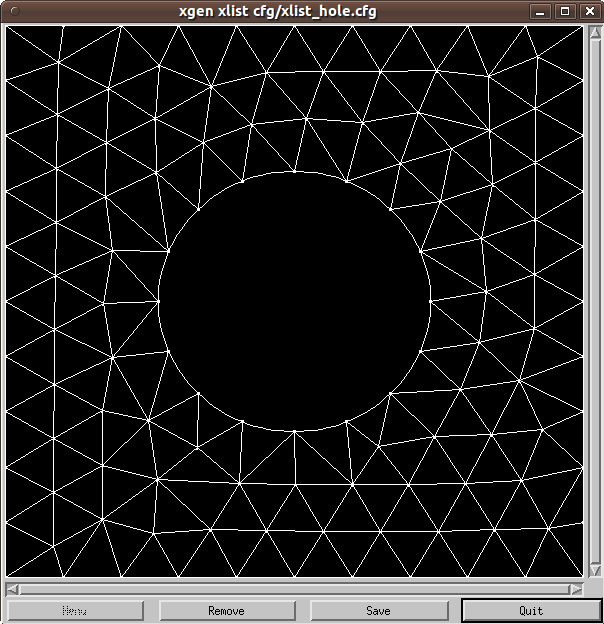
\includegraphics[width=0.6\textwidth]{xgen-7.png}
  \end{center}
  \vspace{-6mm}
  \caption{Sample geometry corresponding to the above input file.}
  \label{fig:7}
  \end{figure}


  \section{Creating Custom Projects} \label{new-project}

  In the previous section we saw how to enter the geometry 
  via a positively oriented list of lines and/or circular arcs.
  In fact, this was just one specific application (called "xlist")
  that consists of less than 50 lines of code (incl. comments). 

  To create a custom project such as "xlixt", one needs to define 
  a descendant of a basic class Xgen. Let us paste the 
  code of the class "xlixt" here for illustration: 

\begin{verbatim}
/*
 *   class xlist:
 *   general polygonal domain with possibly curved edges
 *   see cfg/xlist_curved_6.cfg for an example of input file
 */

class xlist: public Xgen {
  public:
  xlist(char *cfg_filename, bool nogui, int nsteps, bool overlay) 
        : Xgen(nogui, nsteps, overlay) {XgInit(cfg_filename);}
  virtual void XgReadData(FILE *f);
};

// Boundary edges have the following format:
// <marker start_x, start_y, subdivision, angle>
// where angle = 0 for straight edges and angle != 0 for curved.
// New component is introduced with '='.
void xlist::XgReadData(FILE *f) {
  int marker, subdiv, end = 0;
  Point a, b, c;
  double angle;
  char test[20];

  while(Get(f, &marker)) {
    if(!Get(f, &a.x)) XgError("Couldn't read a starting point.");
    if(!Get(f, &a.y)) XgError("Couldn't read a starting point.");
    if(!Get(f, &subdiv)) XgError("Couldn't read a subdivision number.");
    if(!Get(f, &angle)) XgError("Couldn't read an angle.");

    // Closing a boundary loop.
    XgCreateNewBoundaryComponent();

    XgAddBoundarySegment(marker, a.x, a.y, subdiv, angle);
    c = a;
    while(end = !Get(f, test), (end || test[0] == '=') ? false : true) {
      marker = atoi(test);
      if(!Get(f, &b.x)) XgError("Couldn't read a starting point.");
      if(!Get(f, &b.y)) XgError("Couldn't read a starting point.");
      if(!Get(f, &subdiv)) XgError("Couldn't read a subdivision number.");
      if(!Get(f, &angle)) XgError("Couldn't read an angle.");
      XgAddBoundarySegment(marker, b.x, b.y, subdiv, angle); 
      a = b;
    } 
  }
}
\end{verbatim}
This code can be found in the file {\tt src/main.cpp} starting 
with line 199. The method {\tt XgReadData()} reads data from 
a user-supplied text file and uses an elementary function 

\begin{verbatim}
  XgAddBoundarySegment(marker, a.x, a.y, subdiv, alpha);
\end{verbatim}
to create an arbitrary geometry. The function {\tt XgAddBoundarySegment()}
adds a new segment with boundary marker "marker", starting point "a", 
subdivision "subdiv" and angle "alpha". New boundary component (loop) is
created with

\begin{verbatim}
  XgCreateNewBoundaryComponent();
\end{verbatim}

  \noindent
  After creating a new class, add the following three lines into 
  the main() function of the file src/main.cpp, to make sure that 
  the class' name can be used as a command-line parameter:
  \begin{verbatim}
  if(!strcmp(argv[1], "xlist")) {
    xlist X(argv[2]);
    XgMainLoop(&X, argc, argv);
  }
  \end{verbatim}
  That's it! 

  \section{Mesh Output Format} \label{out_form}

  By default, XGEN creates meshes in Hermes2D native format (http://hpfem. org/hermes).
  This can be changed by overriding the virtual method {\tt XgUser Output()}.
  The mesh with the circular hole generated in the previous 
  section can be found in {\tt meshes/xlist\_hole.mesh}. The mesh 
  file contains four parts: {\tt vertices}, {\tt elements}, {\tt boundaries}, and 
  {\tt curves}:

  \begin{verbatim}
# XGEN mesh in Hermes2D format
# Project: cfg/xlist_hole
# Edges are positively oriented

# Vertices:
vertices =
{
  { 0, 0 },
  { 0.3, 0 },
  { 0.6, 0 },
  .
  .
  .
  { 0.228144, 2.8167 },
  { 0.165974, 0.244247 },
  { 0.247855, 0.761208 }
}

# Elements:
elements =
{
  { 40, 41, 63, 0 },
  { 41, 42, 75, 0 },
  { 42, 43, 68, 0 },
  .
  .
  .
  { 89, 59, 94, 0 },
  { 68, 109, 42, 0 },
  { 42, 109, 75, 0 }
}

# Boundary markers:
# (bdy_vertex_1 bdy_vertex_2 edge_index)
boundaries =
{
  { 0, 1, 1 },
  { 1, 2, 1 },
  { 2, 3, 1 },
  .
  .
  .
  { 53, 54, 5 },
  { 54, 55, 5 },
  { 55, 40, 5 }
}

# Circular arcs:
# (bdy_vertex_1 bdy_vertex_2 central_angle)
curves =
{
  { 40, 41, -22.5 },
  { 41, 42, -22.5 },
  { 42, 43, -22.5 },
  .
  .
  .
  { 53, 54, -22.5 },
  { 54, 55, -22.5 },
  { 55, 40, -22.5 }
}
  \end{verbatim}

  \section{Saving and Loading Points}

  Grid points can be saved using the button ``Save points'' in "Menu".
  To load points, use buttons ``Init'' and ``Load''.
  The output file only contains points coordinates as two
  numbers per line. While loading, points that are checked to be
  out of the domain are ignored. 

  \section{XGEN Configuration File}
   
  Upon execution, XGEN attempts to open the file
  .XgenConfig in the current directory. This file 
  can be provided by the user and it contains 
  the following defaults:

  \begin{verbatim} 
# Path to directory with point sets:
points/
# Path to directory with meshes:
meshes/
# SubLoopsNumber:
100
# Initial size limit:
600
# Boundary redraw interval:
200
# Time step change ratio:
0.75
# Zoom ratio:
0.95
  \end{verbatim}
  Variables that are not read from this file are set to some default values.
  Here the points and mesh file paths specify where the points and mesh 
  files are stored, respectively. SubLoopsNumber is the number of
  points to be moved before returning control to the Window Manager.
  The next value is the size of the window when placed on the screen.
  The shape of the window is determined according to the shape
  of the triangulated domain by the generator itself. BoundaryRedrawInterval
  is the number of points to be moved before the boundary is
  redrawn. TimestepConst is a number between 0 and 1 that defines the change of
  the time-step after pressing ``Timestep inc'' and ``Timestep dec'' in ``Menu''.
  The last variable ZoomRatio has a similar meaning in context of zooming.

  \section{Visualizing Meshes with Hermes2D}

  The easiest way to visualize an XGEN mesh is to copy the mesh file into 
  the directory ".../hermes/hermes2d/tutorial/01-mesh" in the Hermes repository
  as "domain.mesh", comment out local refinements
  in the main.cpp file, build the example again typing "make" in its directory, and 
  run "mesh". Then click into the graphics window containing the mesh, and press 's'
  -- this will save a BMP image on the disk. An example for the above GAMM channel
  project is shown in Fig. \ref{fig:hermes}.

\newpage

  \begin{figure}[!ht]
  \begin{center}
  \includegraphics[width=0.8\textwidth]{xgen-6.png}
  \end{center}
  \vspace{-6mm}
  \caption{XGEN mesh visualized in Hermes2D.}
  \label{fig:hermes}
  \end{figure}

  \section{Additional examples}

  The file src/main.cpp contains a few more sample descendants which 
  can be tried via:

  \begin{verbatim}
    ./xgen xsquare cfg/xsquare.cfg &
    ./xgen xhole cfg/xhole.cfg &
    ./xgen xcirc cfg/xcirc.cfg &
    ./xgen xstep cfg/xstep.cfg &
  \end{verbatim}


  \hbox{} \hfill Pavel Solin, May 1995 (updated December 2010)


\end{document}









































